\chapter{Design-Implementation}
\label{chap:design} 

\section{Introduction}

This chapter describes the design, implementation of a human in the loop verification based annotation system. From a users perspective the process is a collaboration between user and a machine learning model, the interface is similar to a diagram editor where a user verifies and corrects object detection predictions.

The implementation is split into three parts, a web based client, training processes running on machines with powerful \gls{GPU}s and a server acting as an intermediary storing image data, user actions and parameters of trained object detection models.


\section{Annotation methodology}

\subsection{Verification based annotation}

\begin{figure}[h!]
  \centering
  \includegraphics[width=1.0\linewidth]{figures/annotation/penguin_refine.pdf}
  \caption{Illustration of a human annotator refining a set of bounding box predictions }   
  \label{fig:penguin_refinement}
\end{figure}

At the core of the user interface is the use of an object detector seamlessly providing immediate feedback on images viewed by the user. When a previously unedited image is opened, the model simply provides the set of predicted detections which are presented for verification to the user. 

In the first implementation, this was a manual operation where a user viewing an image could click a button to retrieve model predictions. This adds an unnecessary action, although it does make it apparent to the user where the annotations came from. One downside to the seamless auto detection and review interface is that it is not necessarily obvious if the annotations being viewed are the result of model predictions or user inputs.

An illustration of the annotation process is shown in figure \ref{fig:penguin_refinement}, showing the user refining a set of bounding box annotations. The diagram illustrates the main operations available to the annotator, which are:

\begin{itemize}
    \item {\bf Transform bounding box}
An inaccurate bounding box can be corrected by clicking and dragging a corner; or to move it's centre, by clicking on the box as a whole and dragging it, the scale may also be adjusted at the same time by scrolling the mouse wheel.
    \item {\bf Confirm weak detection}
If the \emph{review} mode is activated, detections of weak confidence will show with dotted lines. I use a two confidence level threshold system (see section-\ref{sec:thresholding}). A user may then click on the box to confirm it as an annotation.
    \item {\bf Delete box}
Any false-positive prediction from the object detector which meets the threshold as a high confidence detection can be deleted by selecting the box (by clicking on it) and pressing a key. 
    \item {\bf Draw box}
For objects in the image completely missed by the object detector, the user may draw a box by holding a key then clicking once on one corner, and again on the other.
    \item {\bf Submit image}
Once the image has been corrected to the required standard, the user may then submit the annotated image.
\end{itemize}

Some of the operations above may be conflated, for example low confidence predictions are sometimes not localised well - so the user may transform the bounding box at the same time as confirming the weak detection.

\subsection{Reviewing images}

In crowd sourcing image annotation software, quality assurance is usually performed using cross verification where  either multiple users annotate the same images, or each image passes a set of checks performed by other users before the quality is deemed acceptable. Verification prevents malicious or incompetent users to spoil the data and provides some assurance that the end result is of high quality. In this work I prototyped the idea of using the trained model to assist in with quality assurance (a) finding images to review (see section-\ref{sec:example_selection}), and (b) illustrating inconsistencies with the trained model.

When a previously annotated images is opened, the existing annotations are matched with model predictions, and interface functions similarly to a diff viewer, but for image. Matches are determined by a greedy matching process as used for evaluating object detection, described in section-\ref{sec:evaluation_metrics}. The user can view these changes using by toggling the \emph{review} mode on and off. This functions in a similar method to the initial refinement process where the \emph{review} mode is used to show detections of weak confidence. 

Where model predictions differ from the provided annotations a dotted outline is shown on the model's predictions. This highlights annotations where the localisation differs from model predictions, as well as potentially missed annotations. A confidence score is also shown on existing annotations, highlighting annotations for attention which are either missed by the model, or potentially errors in annotation.

The difficulty faced with using the trained model to determine annotation inconsistency, is that the model tends to over-fit the training data. In order to adequately use a trained model for this purpose the image must not be one used directly in the training process. With the current design, this restricts the use to images in the validation set; in future the plan is to use K-fold cross validation, such that each image is left out of training with at least one model. 

It is anticipated this form of quality assurance will prove more useful with a larger number of training examples and thus more accurate object detection models. It may be useful as just one part of a quality assurance system, allowing a user to quickly identify parts of an image which require attention. Further work is required before these ideas can be evaluated properly (and in this thesis I make no attempt), this will likely occur with application to larger scale annotation tasks.

\subsection{Single or few class annotation}
\label{sec:single_class}

While the object detection model used behind the scenes supports multiple classes, the focus of the annotation tool has been on single or few-class annotation. The primary reason is that training a high quality object detector for a given class requires a certain number of examples. If the focus is placed on a single class, the user can annotate more images of that class and thus the model can provide accurate detections sooner, and provide much better assistance the user. It is also anticipated that an object detection model can learn to detect examples of a single class at a high accuracy much faster than it can when training in a multi-class setting. I test this hypothesis in \ref{sec:multiclass} and show that it is very likely this is the case.

With appropriate preparation, annotating a single class at a time should enable a larger number of examples of that class in a shorter period. This is highly dependent on the dataset and the preparation before annotation begins. Some level of pre-sorting (for example by using datasets already labelled for classification) or image selection becomes crucial if classes are very sparsely distributed in the input images; for example if there are a lot of classes, but only a hand-full in any particular image.

The datasets used in this work are either single or few-class, with multiple instances per image; with the exception of the \emph{scallops} dataset, where despite being a single class annotation the instances are sparsely distributed amongst the images.

Multi-class datasets can be annotated one class (or small groups of classes) at a time, however depending on the nature of the data (such as the sparseness of the examples of each class), working this way might be undesirable. As a result it seems likely that this kind of annotation best suits the kind of dataset with many examples of the same class, or the same kind of application in each image. Examples might be counting wildlife or applications for annotations robotics where the task to be performed is similar on every image.


\subsection {Confidence thresholding}
\label{sec:thresholding}

Choosing the confidence threshold is an important parameter for inference using an object detector. The consequence of an incorrect detection threshold is extra work for the annotator, either having to delete too many false positives or be left with too many boxes to draw. Many times, especially with difficult image detection problems an weak detector will produce many detections (some true positives, some false positives). The weak detector will not be able to separate these detections by confidence value. Using human verification there exist some obvious strategies to separate the true positives from the false positives, while still not missing too many objects altogether. 

\begin{itemize}
    \item Set a low detection threshold and have the user delete false positives
    \item Set a low detection threshold and have the user select true positives
    \item Set a high detection threshold and have the user draw boxes around missed detections
\end{itemize}

Each of these strategies has a valid place. If detections are so noisy and if the location predictions are very noisy (for example when the detector is very weak, such as near the start of the process) - having the user draw boxes is often the only option. Some of these strategies are amongst used by \cite{Konyushkova2017} which attempts to solve this problem differently, by attempting to automatically determine the best interface for a given image.

Deleting false positives is often the best option if true positives outnumber the false positives, or if the false positives are easy to select (if they're grouped together, for example). Selecting true positives is often the best option if the false positives outnumber the true positives. 

Another strategy exists, which has the best of both worlds. Two thresholds can be used, a high confidence threshold can be used for eliminating false positives (such that when using this threshold the number of false positives is low). Detections between the high and low confidence thresholds can be considered for selection as true positives (such that the number of true positives requiring selection is low).


\begin{figure*}[h]
\centering
\begin{subfigure}[t]{0.5\linewidth}
  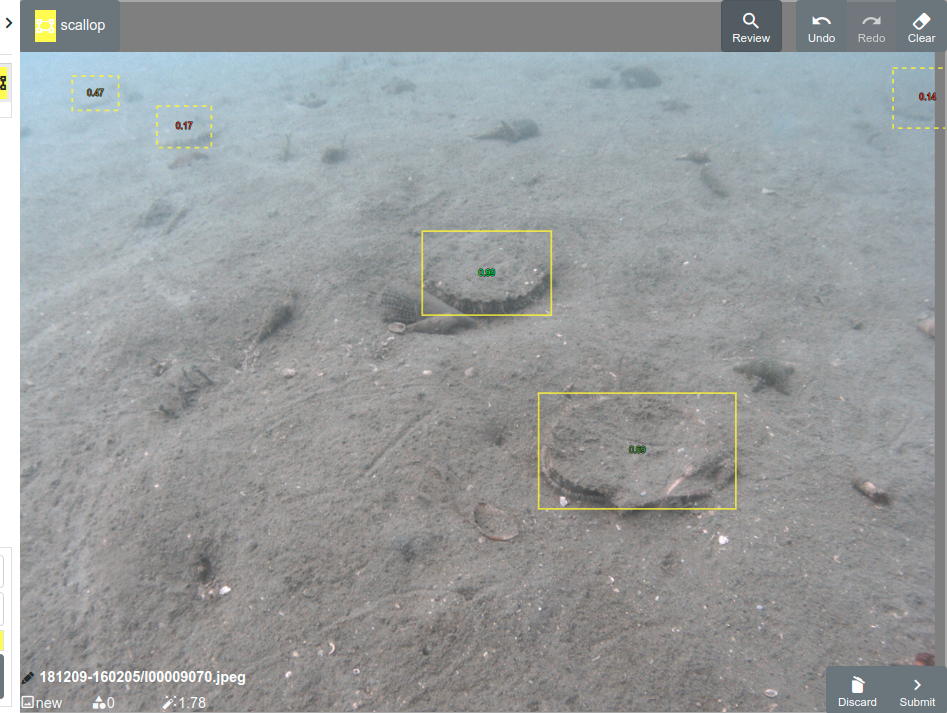
\includegraphics[width=1.0\linewidth]{figures/annotation/scallop/review_mode.png}
  \caption{}
\end{subfigure}%
\begin{subfigure}[t]{0.5\linewidth}
  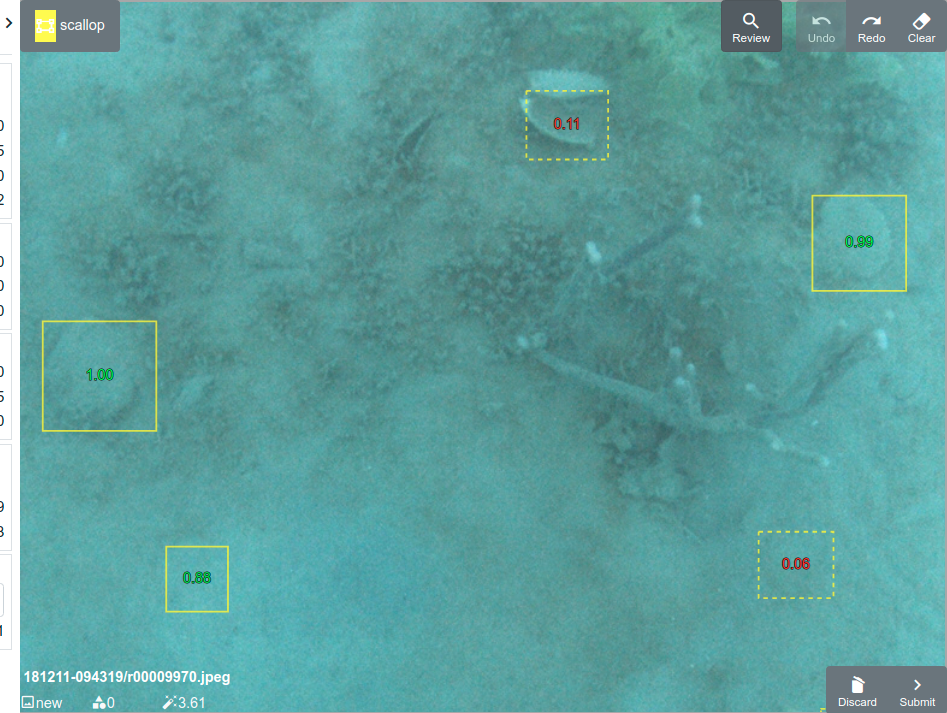
\includegraphics[width=1.0\linewidth]{figures/annotation/scallop/false_positive.png}
  \caption{}
\end{subfigure}%
\caption{Review mode used on two fresh images from the scallop dataset, (a) showing an ideal case (b) showing an image with a high confidence false positive among low confidence detections}
\label {fig:scallop_review}
\end{figure*}


I provide a key which toggles between showing the detections in the mid range between the two thresholds, when the key is held a click is used to confirm a detection as a true positive. I term this toggle ``review mode''.  An example showing the mechanic of this can be seen in figure \ref{fig:scallop_review}. In one image the ideal situation is shown where three scallops are detected in the background (with low confidence), where otherwise they might have been ignored. In the other, a less useful case where the low confidence detections are false positives, and one of the high confidence detections is also a false positive, despite this the user saves time by ignoring the other low confidence detections.

The other advantage of this strategy are that it can bring the annotators attention to areas of the image which may have gone unnoticed. I have noticed in particular with the underwater scallop images that the detector usually did a good job at bringing attention to the more uncertain scallop instances. It also provides useful feedback to the annotator of the progress of the current object detector. 

During training it can be seen that the confidence levels provided by the object detector vary with regard to training time. This is a known property of neural network classifiers \cite{Guo2017}.

In future I would like to investigate calibration of thresholds using validation so that the user has nothing to do with this. This can be done by continually adjusting thresholds to match a certain ratio of false positives to false negatives (the desired ratio to be set by the user), alternatively prediction confidence itself can be calibrated to attempt to provide more consistent values. Confidence scores can be calibrated by scaling scaling outputs prior to applying softmax normalisation \cite{Guo2017}. For the purpose of object counting I use the former method to select thresholds. In order to provide the most unbiased estimate of counts the confidence is selected to give an equal ratio of false positives to negatives.
 


\subsection{Example selection}
\label{sec:example_selection}

While not the core focus of this work, active learning and example selection is complimentary to verification based annotation, and I have implemented a number of simple metrics for example selection. While there exist very recent measures of uncertainty for object detection (for example using Bayesian \gls{NMS} \cite{Harakeh}, ensembles \cite{Le2018}, or test time augmentation \cite{Wei2018}), there are also a number of very simple metrics which I have found useful in different kinds of workflows. 

Verification based annotation also overlaps in purpose with active learning, both attempt to remove the burden of labelling all the easy cases in a dataset. Active learning seeks to have the annotator label the most informative images via. example selection, and verification based annotation attempts to achieve the same thing via. automatically label the easy cases so the human annotator does not have to.

Some image sets more sparsely populated with examples however benefit much more clearly, for example in the scallop imagery where a large proportion of the images contain no scallops, and it seems likely that given plentiful negative examples that images with multiple scallops are more informative. 

A sample of non-annotated images are detected at each training iteration and images with large detection score are presented to the user first. Images with false positives will also score highly here, however false positives are also informative for training. This would also be an important workflow for adding new object classes to existing datasets where it becomes important to find instances of new examples in old images.


\begin{itemize}
\item {\bf Detection score. }

For this I use the sum of squares of the confidence scores, $ \sum_(p \in detections){ p^2 } $ where $p$ is the confidence for a given detection. 

    \item {\bf Count variation. }
Used with object counting datasets, where the sensitivity of the count in each image is used. Images with the widest difference in count at two thresholds are selected first, the two thresholds determined on the validation set to give $ \pm 10\% $ counts.
    \item {\bf Frame variation. } 
In time sequence and video datasets, the variation in count between nearby frames can be used to estimate uncertainty. For this I use the different between a frame and a running average for a window centred around that frame. For this, the metric is computed after predictions for all frames are computed, and counts estimated.
    \item {\bf Training error. }
Use of the loss from training was proposed for the purpose of finding training images with error. Initial experiments with this indicate the object detection models manage to fit images even with the most obvious mistakes with low loss, making this form of example selection less useful. In future using a k--fold cross-validation training ensemble is proposed such that each image is left out of training for at least one model, allowing an unbiased comparison with at least that model.
\end{itemize}


\section {User interface}

The user interface of the system resembles a diagram editor, where annotation shapes (boxes, circles, polygons) can be drawn over an image and manipulated in the usual ways. Shapes can be moved by selecting and dragging, resized by scrolling the mouse wheel or by dragging control points. 

Multiple annotations can be selected together using a rectangle select, and moved together. In particular this saves a lot of time when the model creates excessive extraneous detections. This occurs frequently when an image contains objects of a scale previously unseen, or containing content from a distribution previously unseen by the model. \gls{CNN} models are known to produce false positives on out of distribution images \cite{todo}. For example in the scallop imagery when querying predictions on an image containing a (previously unseen) diver.

\subsubsection {Navigation}

Navigation is crucial to being able to effectively examine an image (and thus annotate it well). The ability to zoom into a portion of an image to view it more closely and see details is important, this is particularly important for parts of an image with higher uncertainty. Equally important is the ability to zoom out to view the whole image, to check for missed details. 

I use a familiar interface controls most similar to Google Maps \cite{todo}, where panning is achieved by clicking and dragging and zooming is achieved by mouse wheel. The zoom centres around the mouse cursor such that the image at the mouse cursor is fixed.

Limited functionality is implemented for navigating video sequences, it is possible to view a few frames forward and backwards using keyboard shortcuts. This helps avoid ambiguity from an annotation perspective, often in a video sequence if something is unclear from a single frame it is possible to resolve that ambiguity by viewing back or forward in time. An example of this is in the \emph{seals} dataset (described in chapter \ref{chap:datasets}) where identifying a pup next to a mother is often somewhat ambiguous, but viewing the motion over time usually resolves the ambiguity.

\subsection {Browsing and sorting}


In addition to the metrics used for example selection, I found it useful to provide ways for a user to rank images according to various criteria.

\begin{itemize}
    \item {\bf Modification time.}
Select images least recently modified for reviewing.
    \item {\bf Image creation time. }
Select images in creation time, useful for comparing images in time. One example is synchronising images taken concurrently from different streams, for example seal counts at Scott Base captured by two different cameras.
\end{itemize}




\section {Implementation}

\subsection{Server and client}

\begin{figure}[h!]
  \centering
  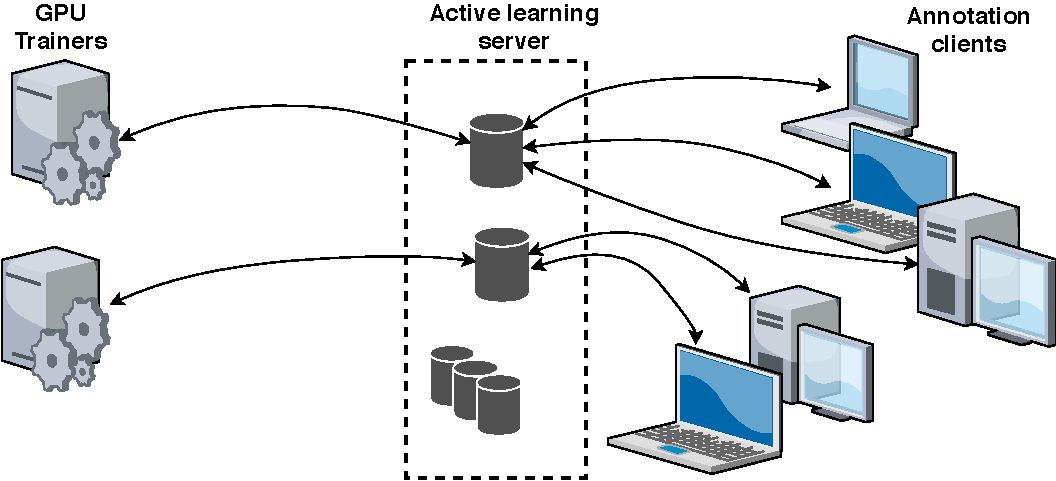
\includegraphics[width=1.0\linewidth]{annotation/connectivity.pdf}
  \caption{Connectivity of the annotation system}  
  \label{fig:connectivity}
\end{figure}

The system can be broken down into three parts running separately but communicating. This can be seen in figure \ref{fig:connectivity}. There exists a server process which sits in the middle and acts as a conduit for communication, a store of data and a serialisation of state. The server sits in the middle and communicates with both trainers and clients.

The main reason for splitting server and trainer was initially for practical reasons, the client and server both written in \gls{GHC} Haskell, and the deep learning framework of choice was Pytorch \cite{Paszke2017}. The server and client are written in Haskell, the former running naively, the later compiled to JavaScript using \gls{GHCJS}. The interface uses a \gls{SVG} for display, but in future I plan to switch for \gls{HTML} canvas for faster rendering and simplicity.

Splitting server and trainer does also provide some advantages. It allows the server to act as a portal through which users can work on several datasets. One or many trainers can be shared concurrently or time shared without having to run new instances of the server. 

The current reality is more simple, a single trainer services the server and operates on a first come first served basis. One dataset at a time is trained, until a period of inactivity (no images submitted for $ n $ training epochs). A trainer still services clients working on inactive datasets by providing detection (best models for each dataset are kept in \gls{CPU} memory), but trains on only one dataset at a time. 

Due to the nature of memory management on a \gls{GPU}, and the memory requirements of training we interleave requests originating from clients and training. When a user selects an image, the first action taken is to query the trainer for a set of detections. It is therefore necessary to stop training temporarily, run object detection inference on the image in question, then resume training. In attempt to mitigate the delay, a small number of frames are processed in advance according to the current ordering in use at the time. For larger images, the transmission and decoding of image data in the current system causes more significant visible delay than the response time to the object detection query.

In future it would be an advantage to allow one or more \gls{GPU} processes to be dedicated to serving user requests in the interests of reducing response time. Low response time is important especially for the purposes of interacting with video if skipping forwards and backwards in time (spanning potentially many frames at a time), can occur without unreasonable delay.

\begin{figure}[h!]
  \centering
  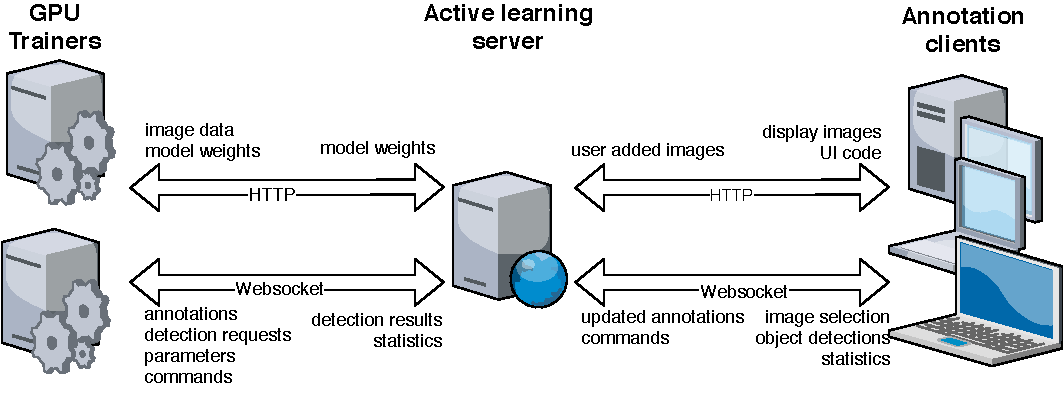
\includegraphics[width=1.0\linewidth]{annotation/data_flow.pdf}
  \caption{Data flow between services for the annotation system}  
  \label{fig:data_flow}
\end{figure}

An illustration of the data flow which occurs between different parties can be seen in figure \ref{fig:data_flow}. Large binary data is shared using \gls{HTTP}, for example model weights and images are distributed this way. Other data is communicated over websocket connections using \gls{JSON} text. Examples of this includes synchronising new annotations, and image statistics, which are continually updated to the client for the purpose of the example selection in active learning.

Image data is stored on the server and transmitted as required to trainer and client. Images are sent to client for viewing and inspection, and to the trainer for training and cached for more efficient loading. 

Models are stored on the server and requested by the trainer as required, for example when starting training on a dataset the trainer requests the previously stored model weights. The trainer also caches copies of weights (as required) of recently used models for the purposes of inference as required by the client for every image opened. Given the large size of data involved in transmitting large images, and also updating model weights, the trainer is suited to exist on the same local network as the server. 



\subsection {User interface}

I provide a web interface for the following reasons:

\begin{enumerate}
    \item No installation
\end{enumerate}
Any system with a web browser will be fine, software utilising complex computer vision and GPU programming libraries is often hard to package for easy installation. A web interface sidesteps these difficulties.
\begin{enumerate}[resume]
    \item Local GPU not required
\end{enumerate}
By running the trainer on another system anyone can use the system without requiring a local GPU. One of the problems with usability from my earlier work was that GPU intensive tasks running on the same computer ruin the responsiveness of a user interface. To my knowledge there is no good way to run a heavy \gls{GPU} intensive processing task at a low priority such that the user interface remains responsive.
\begin{enumerate}[resume]
    \item Enables collaborative annotation/crowd sourcing
\end{enumerate}
A web interface enables a straightforward extension to use for larger scale annotation with multiple users annotating the same dataset. An example can be seen in \ref{fig:connectivity} showing two groups of users operating on the same datasets.


The trade-off for a web interface is in performance, it prevents doing computationally heavy calculation in the client, especially for loading and processing large images. For this work we face no such difficulty, though for example a super pixel based tool for mask annotation would be more challenging. With newer web technologies such as WebAssembly \cite{Haas2017} to run code at near native speeds in a browser, and WebGL shaders for GPU programming.

